\chapter{Tests af system}
\label{bilag:test}
\section{Test af samlet system}
\label{sec:test_samlet}
Testens formål er at udføre en vector network analyse af det samlede system for at finde systemets amplitude-karakteristik og gruppeløbetid. 
Det samlede system består af modtageren af indgangssignalet, anti-aliasing filtrene for den ene kanal, Tiva-kittet med EMP board og microcontroller, DAC, rekonstruktionsfilteret for den ene kanal og udgangskredsløbet. 

\subsection{Udstyr}
\begin{itemize}
	\item Bode 100 med tilhørende udstyr
	\item Èn computer med Bode Analyzer Suite installeret
	\item To oscilloskop-prober
	\item Skillekondensator
\end{itemize}

\subsection{Fremgangsmåde og forsøgsopstilling}
Opsæt Bode 100 uden noget tilsluttet. 
Åben Bode Analyzer Suite, og vælg en Gain/Phase-analyse under Vector Network Analysis. 
Analysen sættes op med følgende indstillinger:
\begin{multicols}{2}
\begin{itemize}
	\item Startfrekvens: 10 Hz
	\item Slutfrekvens: 50 kHz
	\item Minimum 401 data points
	\item Source level: 0 dBm
	\item Attenuator på receiver 1 \& 2: 10 dB
	\item Receiver bandwidth: 100 Hz
	\item External reference på CH1 \& CH2
\end{itemize}
\end{multicols}
Vælg Trace 1 til Magnitude (dB) og Trace 2 til Tg. \newline
Med Bode Analyzer suite laves en kalibrering af Bode 100, når udgangen og indgangene på Bode 100 er koblet sammen. 
Skillekondensatoren skal være på udgangen. \newline
Opsæt det samlede system som vist i bilag \ref{bilag:diagram}. 
Bode 100's udgang med skillekondensator og CH1 kobles til indgangen på den ene kanal af det samlede system. 
CH2 kobles til udgangen af det samlede system for den tilsvarende kanal. 
Analysen kan nu udføres. 

\subsection{Resultat af test}
Datasættet for resultatet af testen kan ses i den vedhæftede fil \textit{'Målinger/Samlet\textunderscore system.csv'}. På figur \ref{fig:tf_tg_samletsystem} kan amplitude-karakteristikken og gruppeløbetiden for det samlede system ses.
\begin{figure}[h]
	\caption{I det øverste plot er amplitude-karakteristikken for det samlede system, og i det nederste plot er gruppeløbetiden.}
	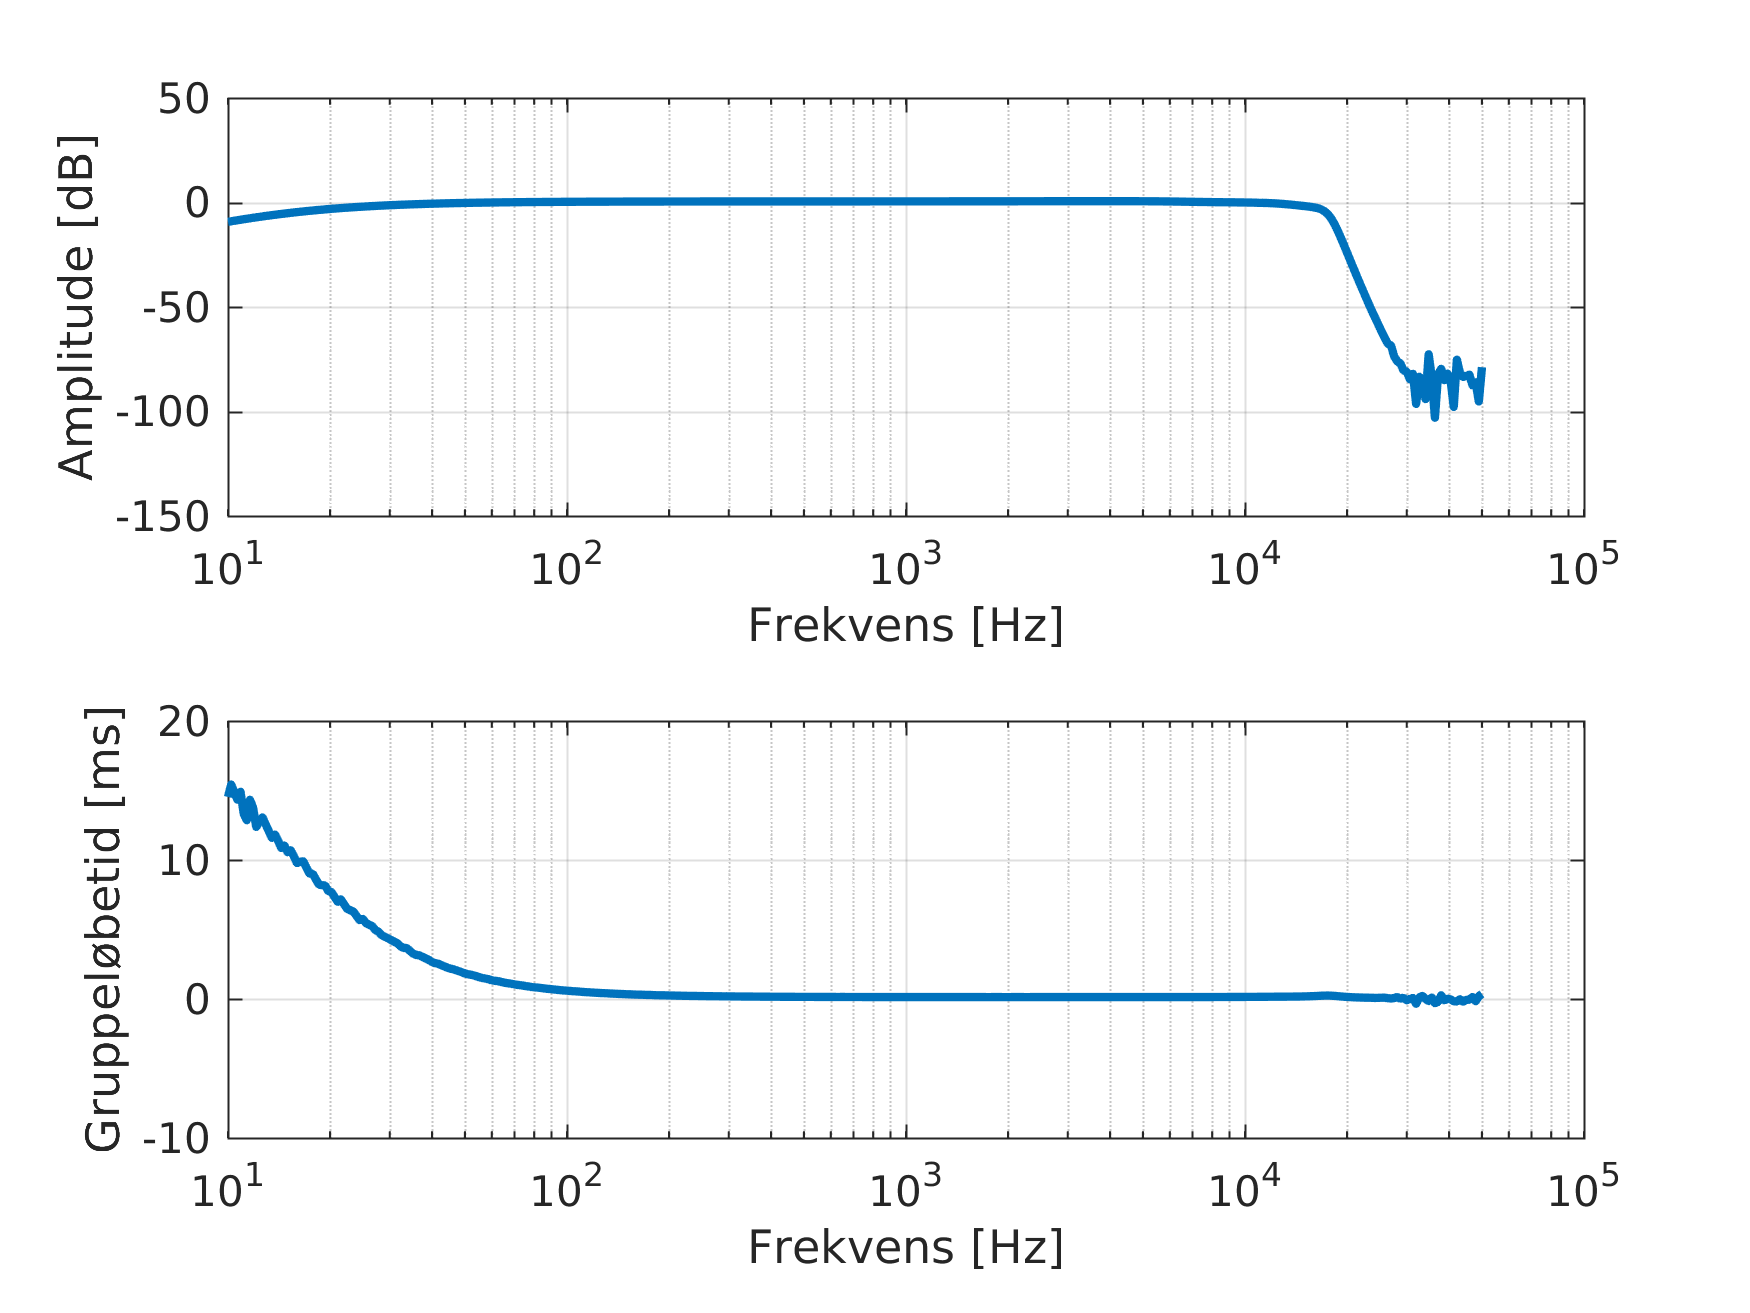
\includegraphics[width=1\linewidth]{matlab/tf_tg_samletsystem.png}
	\label{fig:tf_tg_samletsystem}
\end{figure}

\section{Test af anti-aliasing filter}
\label{sec:test_aafilter}
Testens formål er at finde amplitude-karakteristikken for ét af anti-aliasing filtrene. 

\subsection{Udstyr}
Der skal benyttes det samme udstyr, som til testen af det samlede system i afsnit \ref{sec:test_samlet}.

\subsection{Fremgangsmåde og forsøgsopstilling}
Frem til og med kalibreringen af Bode 100 følger testen samme fremgangsmåde som ved testen af det samlede system i afsnit \ref{sec:test_samlet}. \newline
Opsæt biquads-filtrene i kaskade som vist i bilag \ref{bilag:diagram} i kassen 'Generisk sjette ordens filter'. 
Bode 100's udgang med skillekondensator og CH1 kobles til indgangen på det første biquad filter. 
CH2 kobles til udgangen af det sidste biquad filter. \newline
Analysen kan nu udføres. 

\subsection{Resultat af test}
Datasættet for resultatet af testen kan ses i den vedhæftede fil \textit{Målinger/Filter.csv}. Amplitude-karakteristikken for anti-aliasing filtret er vist på figur \ref{fig:tf_filter}. 

%\begin{wrapfigure}[15]{c}{0.5\textwidth}
%	\caption{\label{fig:fig:tf_filter}Amplitude-karakteristikken for ét anti-aliasing filter.}
%	\centering
%	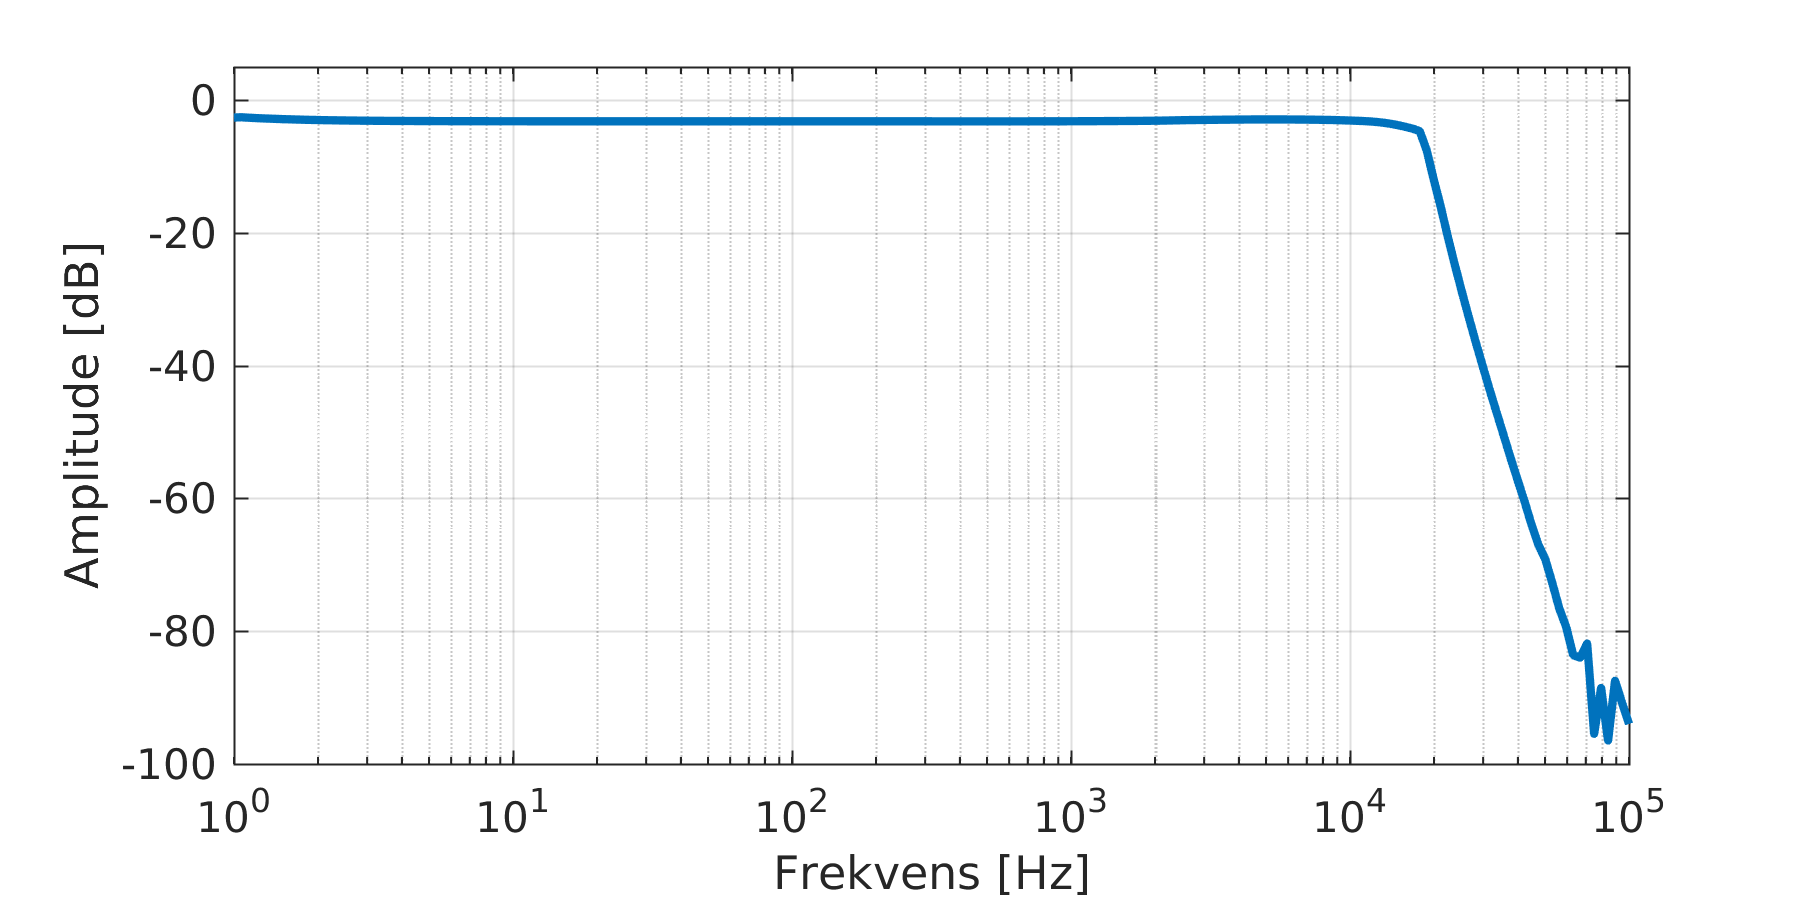
\includegraphics[width=1\textwidth]{matlab/tf_AAfilter.png}
%\end{wrapfigure}

\begin{figure}[h]
	\caption{Amplitude-karakteristikken for ét anti-aliasing filter.}
	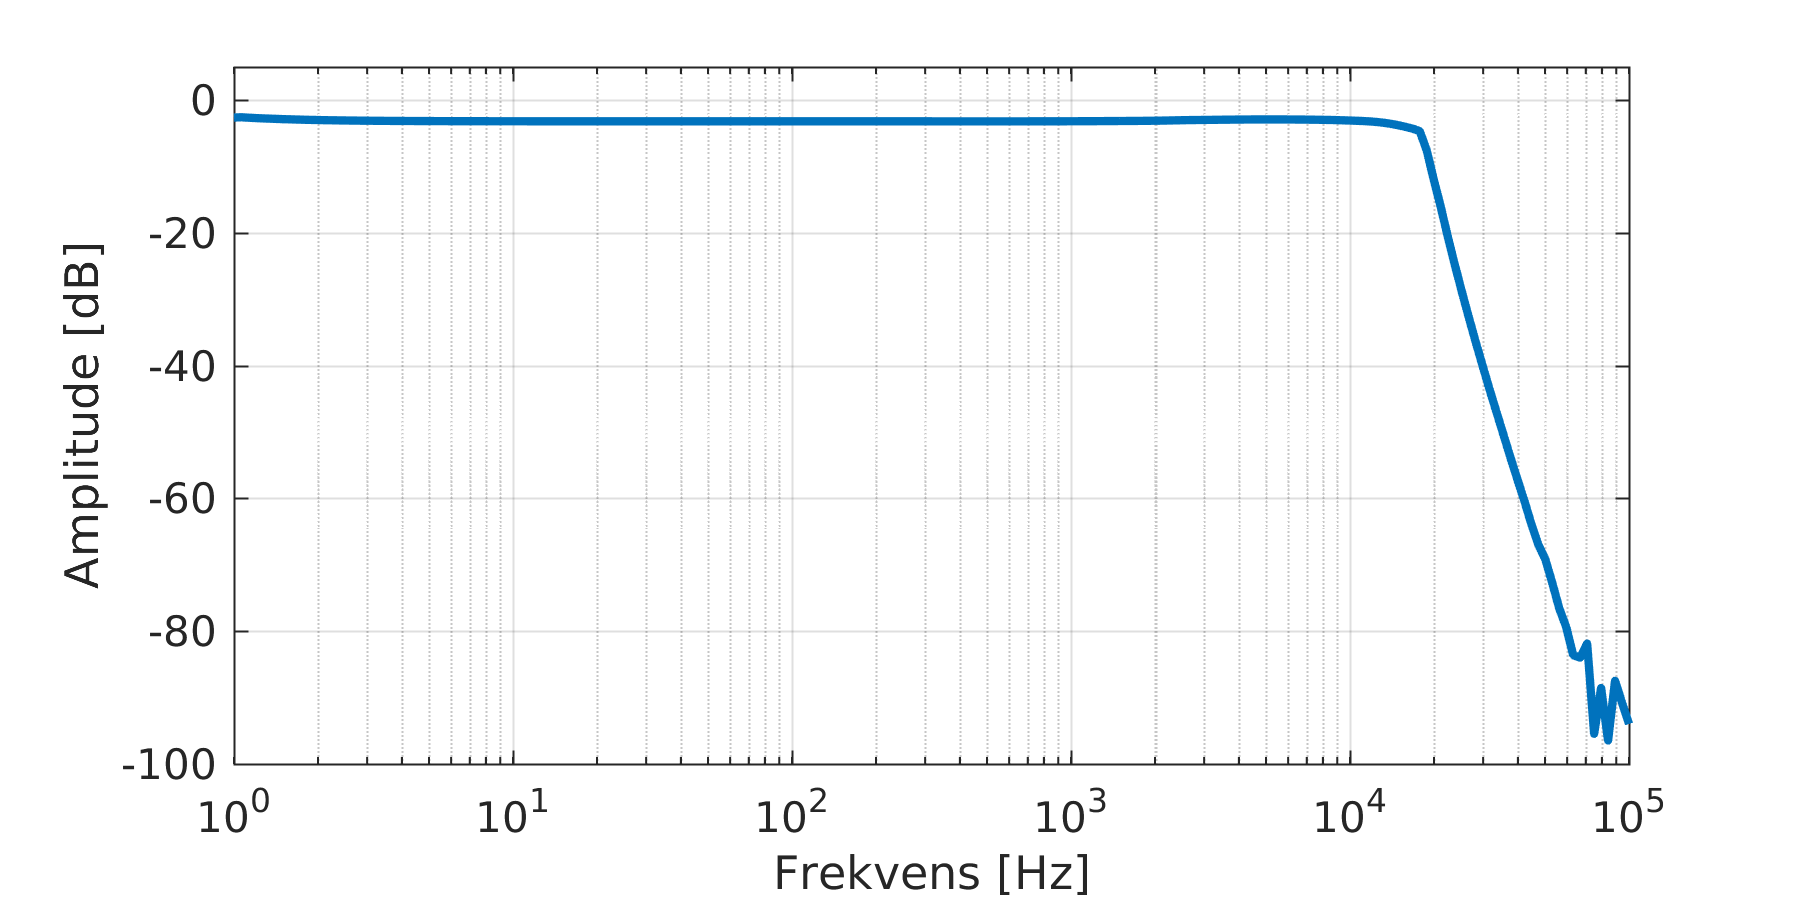
\includegraphics[width=1\linewidth]{matlab/tf_AAfilter.png}
	\label{fig:tf_filter}
\end{figure}